\documentclass[12pt,a4paper,oneside]{article}

\usepackage[utf8]{inputenc}
\usepackage[greek,english]{babel}
\usepackage{alphabeta} 

\usepackage[pdftex]{graphicx}
\usepackage[top=1in, bottom=1in, left=1in, right=1in]{geometry}
\usepackage{hyperref}
\linespread{1.06}
\setlength{\parskip}{8pt plus2pt minus2pt}
\usepackage{fancyhdr}
\widowpenalty 10000
\clubpenalty 10000

\newcommand{\eat}[1]{}
\newcommand{\HRule}{\rule{\linewidth}{0.5mm}}

\usepackage[official]{eurosym}
\usepackage{enumitem}
\setlist{nolistsep,noitemsep}
\usepackage[hidelinks]{hyperref}
 \usepackage[table]{xcolor}



\usepackage{lipsum}
\hypersetup{
    colorlinks=true,
    linkcolor=black,
    filecolor=magenta,      
    urlcolor=blue,
}

\begin{document}

\renewcommand{\contentsname}{Περιεχόμενα}

\renewcommand{\refname}{Αναφορές}

%===========================================================
\begin{titlepage}
\begin{center}

% Top 
\includegraphics[width=0.55\textwidth]{upatras_logo.jpg}~\\[2cm]


% Title
\HRule \\[0.4cm]
{ \LARGE 
  \textbf{PROJECT TΕΧΝΟΛΟΓΙΑ ΛΟΓΙΣΜΙΚΟΥ}\\[0.4cm]
  \emph{Team-plan-v0.1}\\[0.4cm]
}
\HRule \\[1.5cm]



% Author
{ \large
  \includegraphics[width=0.5\textwidth]{logo.png}~\\[2cm]
 
}

\vfill

\textsc{\large Τμήμα Μηχανικών Ηλεκτρονικών Υπολογιστών \& Πληροφορικής}\\[0.4cm]


% Bottom
{\large \selectlanguage{greek}\today}
 
\end{center}
\end{titlepage}
\pagestyle{fancy}
\fancyhead[RO,LE]{Team-plan-v0.1}
\fancyhead[LO,CE]{\includegraphics[width=0.05\textwidth]{logo.png}}
\centering
Ακολουθεί ο πίνακας με τα ονόματα και τα ΑΜ της ομαδάς μας:

\centering
\begin{tabular}{ |p{4cm}|p{4cm}|p{3cm}|}
\arrayrulecolor{gray}
 \hline
 \multicolumn{3}{|c|}{Μέλη} \\
 \hline
 ΕΠΩΝΥΜΟ& ΟΝΟΜΑ & Α.M\\
 \hline
 ΛΙΟΥΜΗΣ   & ΕΥΑΓΓΕΛΟΣ    & 1054325\\
 ΣΧΙΖΑΣ &  ΝΙΚΟΛΑΟΣ & 1054394\\
 ΛΥΡΟΥ & ΔΗΜΗΤΡΑ & 1057774\\
 ΜΠΟΥΡΣΑΛΗΣ   & ΕΜΜΑΝΟΥΗΛ & 1056284\\
\hline 

\end{tabular}


\vspace{7cm}
\raggedright
\textbf{Editors:}
\newline
Νίκος Σχίζας-Δήμητρα Λύρου

\textbf{Contributors:}
\newline
Ευάγγελος Λιούμης-Εμμανουήλ Μπούρσαλης


\vspace{8cm}

\raggedright
\textbf{Εργαλεία:}

    Overleaf
    
    Microsoft Visio(Pert Chart)
    
    TeamGantt(Gantt Chart)

\newpage

%===========================================================

\tableofcontents
\addtocontents{toc}{\protect\thispagestyle{empty}}

\newpage
\setcounter{page}{1}

%===========================================================
%===========================================================

\section{Σύνθεση Ομάδας}\label{sec:intro}
\pagestyle{fancy}
\fancyhead[RO,LE]{Team-plan-v0.1}
\fancyhead[LO,CE]{\includegraphics[width=0.05\textwidth]{logo.png}}

Η σύνθεση της ομάδας μας είναι η εξής:
\vspace{0.5cm}

\begin{tabular}{ |p{4cm}|p{4cm}|p{3cm}|p{3cm}|  }
 \hline
 \multicolumn{4}{|c|}{Μέλη} \\
 \hline
 ΕΠΩΝΥΜΟ& ΟΝΟΜΑ &ΑΡΙΘΜΟΣ ΜΗΤΡΩΟΥ&ΕΤΟΣ ΦΟΙΤΗΣΗΣ\\
 \hline
 ΛΙΟΥΜΗΣ   & ΕΥΑΓΓΕΛΟΣ    & 1054325 &  5\\
 ΣΧΙΖΑΣ &  ΝΙΚΟΛΑΟΣ & 1054394  & 5\\
 ΛΥΡΟΥ & ΔΗΜΗΤΡΑ & 1057774 &  5\\
 ΜΠΟΥΡΣΑΛΗΣ   & ΕΜΜΑΝΟΥΗΛ & 1056284 & 5\\
\hline 
\end{tabular}


\vspace{2cm}
Επίσης, όπως έχει φανει και στην αρχική σελίδα αλλά και σε κάθε σελίδα των παραδοτέων η ομάδα μας θα έχει το εξής λογότυπο:
\newline
\vspace{2cm}
\centerline{\includegraphics[width=0.5\textwidth]{logo.png}}
 
\newpage

\section{Gantt Chart}\label{sec:lit-rev}
\textbf{Παραδοχές για τον σχεδιασμό των διαγραμμάτων:}
\vspace{2mm}
\newline
 Ως ημερομηνία έναρξης θεωρούμε την 9/3/21 καθώς τότε συγκροτήθηκε η ομάδα μας. Λαμβάνοντας υπόψιν τις τελευταία ενημερωμένες ημερομηνίες στο eclass του μαθήματος θεωρήσαμε τα εξής παραδοτέα:
 \newline
 
 \centerline {\textbf{1o} Παραδοτέο: 21/03}
 \centerline  {\textbf{2o} Παραδοτέο: 07/04}
 \centerline  {\textbf{3o} Παραδοτέο: 25/04}
 \centerline  {\textbf{4o} Παραδοτέο: 12/05}
 \centerline  {\textbf{5o} Παραδοτέο: 30/05}
 \centerline  {\textbf{6o} Παραδοτέο: 06/06}
 \vspace{2mm}
 Ως φοιτητές τα μέλη της ομάδας μας εργάζονται τόσο Σάββατα οσο και Κυριακές. Επίσης, ως ορόσημα(milestones) θεωρήσαμε τις ημερομηνίες του κάθε παραδοτέου. Τα ορόσημα(milestones) διακρίνονται απο το εικονίδιο \space
   
\includegraphics[width=0.027\textwidth]{milestone.png}
 
\begin{center}

  \makebox[\textwidth]{\includegraphics[width=1.25\textwidth]{Gantt part2.pdf}}
    
\end{center}

\section{Pert Chart}\label{sec:lit-rev}




 
\centerline{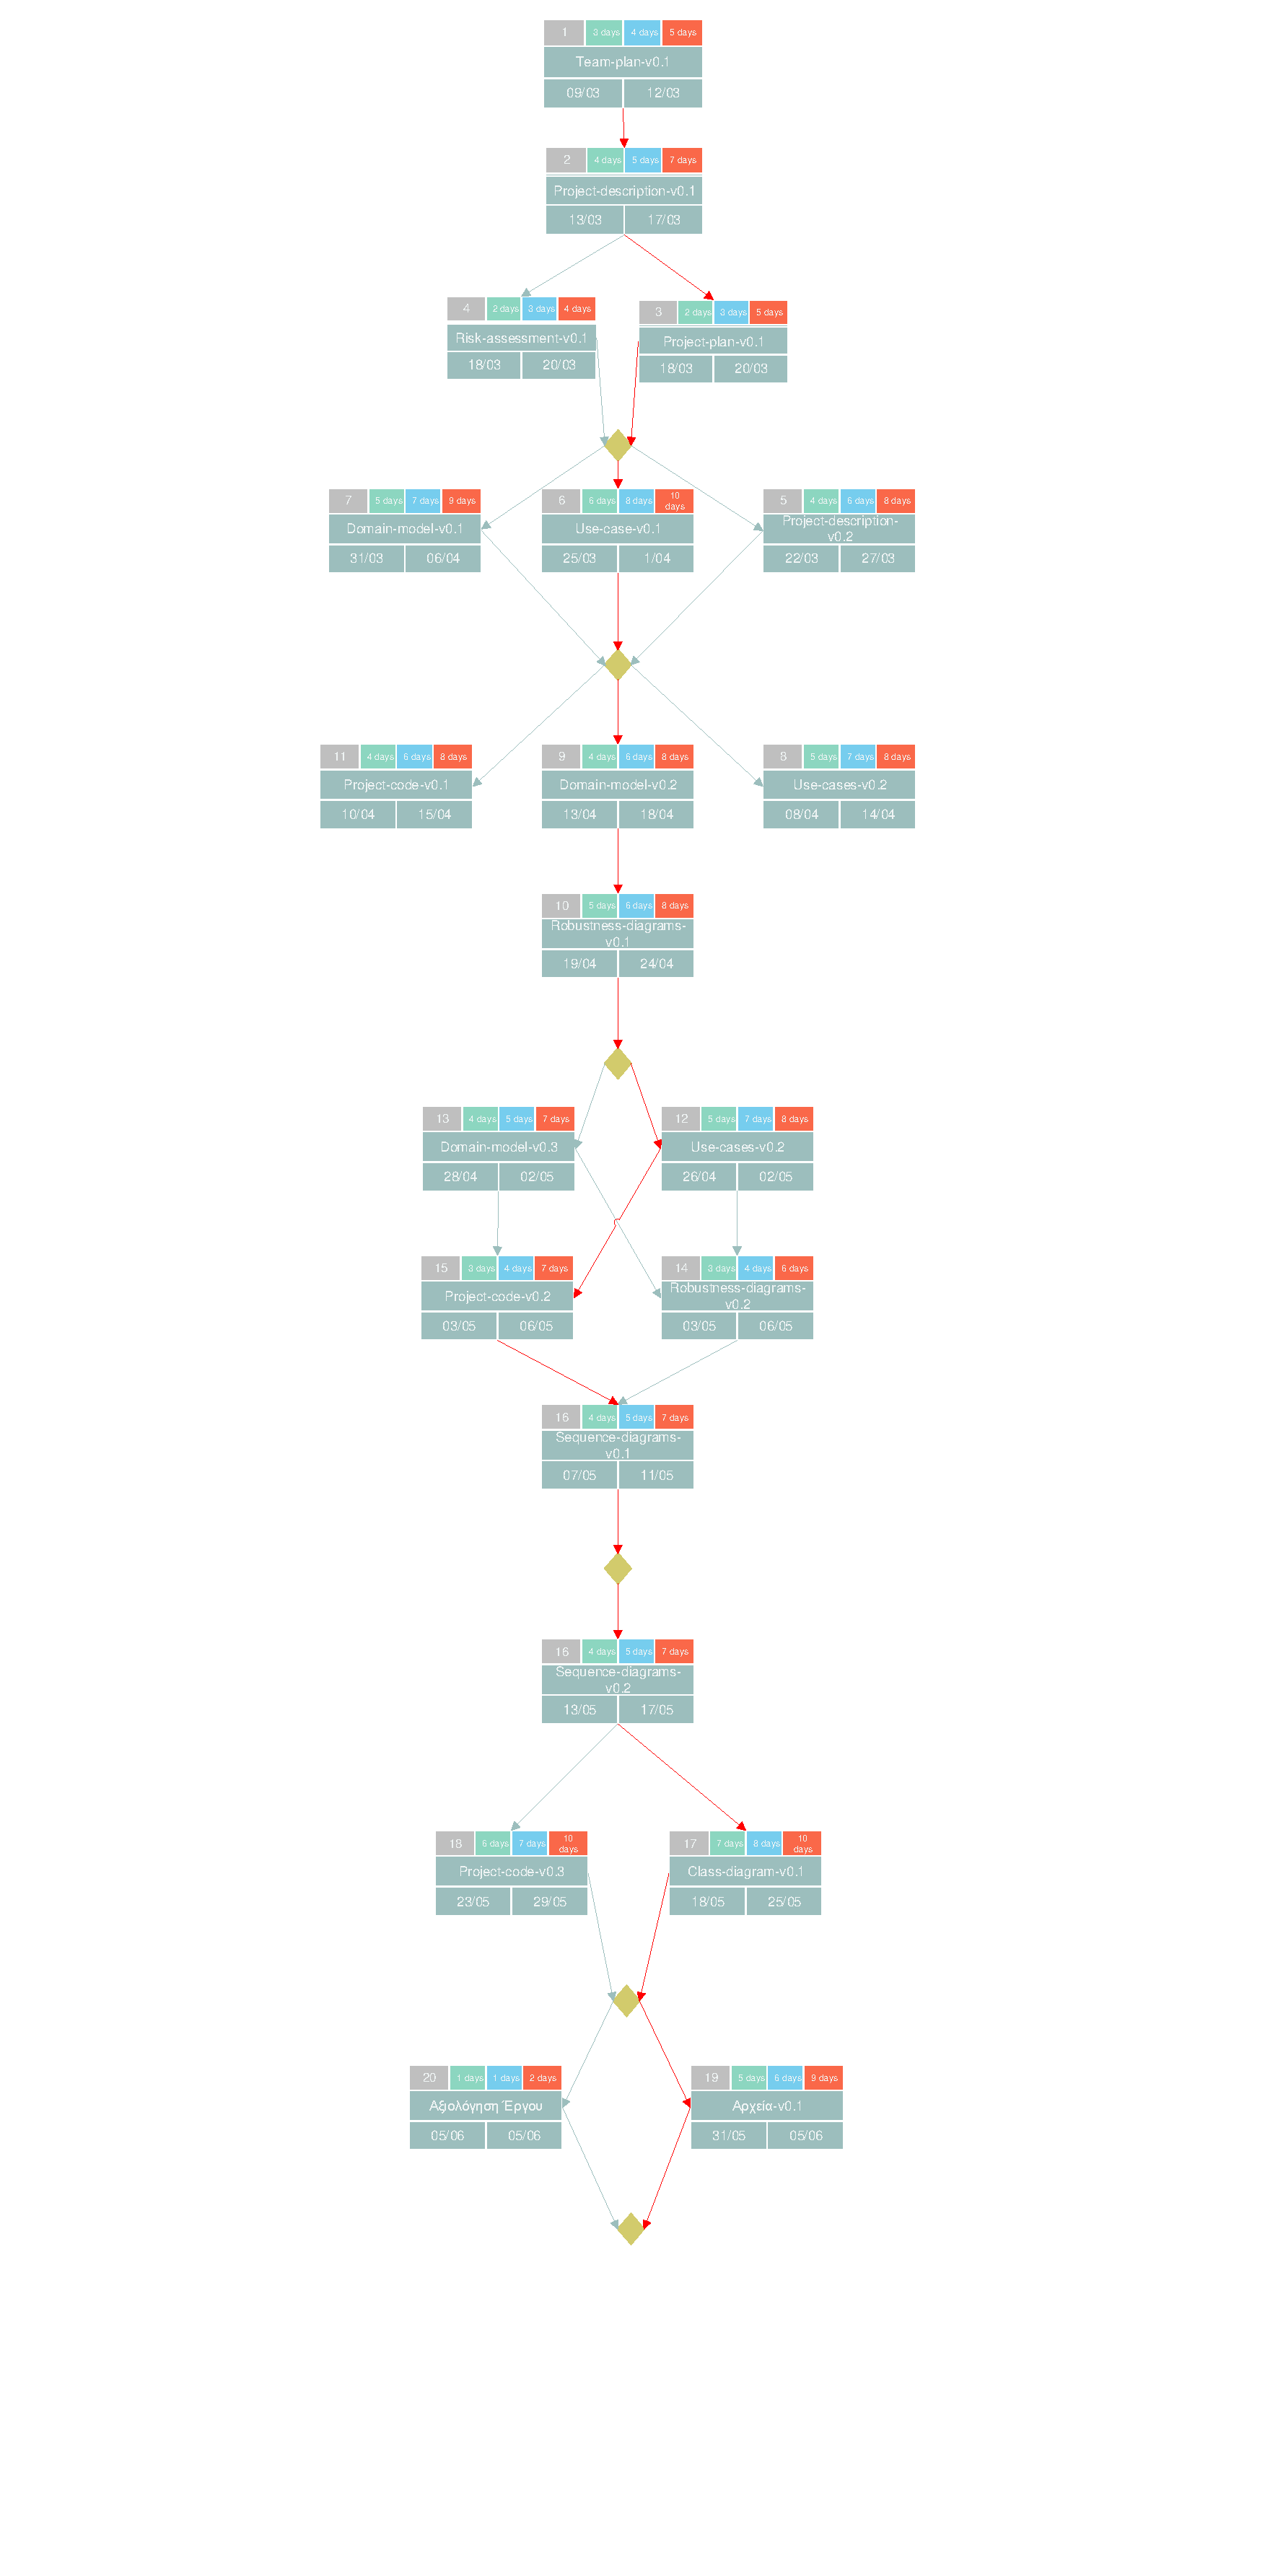
\includegraphics[width=17cm,height=23.7cm]{second try ΤΛ pert chart.pdf}}


\newpage 
\section{Μεθοδολογία}\label{sec:meth}

Θα εργαστούμε έχοντας ως βασική μέθοδο οργάνωσης το SCRUM. Κάθε sprint θα έχει διάρκεια μίας εβδομάδας. Οι συναντήσεις θα έχουν ως  εξής: 
 \begin{center}
Catch-up (Ανά 2 ημέρες) Διάρκεια: 30 λεπτά 

Planning (Στο τέλος κάθε sprint) Διάρκεια: 15 λεπτά 

Review (Στο τέλος κάθε sprint) Διάρκεια: 90 λεπτά 

Refinement (Στη μέση κάθε sprint) Διάρκεια: 30 λεπτά 
\end{center}
 

{Οι ρόλοι θα έχουν ως εξής: }
\vspace{5mm}


\centerline {\textbf{Scrum Master:} Ευάγγελος Λιούμης }

\centerline {\textbf{Product owner:} Νικόλαος Σχίζας }

\centerline {\textbf{Developer:} Εμμανουήλ Μπούρσαλης }

\centerline {\textbf{Developer:} Δήμητρα Λύρου }
\vspace{0.7cm}
Για τις συναντήσεις και την επικοινωνία της ομάδας, χρησιμοποιήθηκε το ZOOM. Για τη διαχείριση των τεχνικών κειμένων χρησιμοποιήθηκε ένας κοινόχρηστος φάκελος στο Microsoft OneDrive. Για την οργάνωση και τη διαχείριση των sprints χρησιμοποιήθηκε το εργαλείο Atlassian Jira. Για την αποθήκευση του κώδικα δημιουργήθηκε ένα repository στο Atlassian Bitbucket. Αν υπάρξουν αλλαγές θα παραδωθεί νέα έκδοση (v0.2). 

\section{Εργαλεία}\label{sec:res}

Μια πρώτη εκτίμηση που κάνει η ομάδα μας για τα εργαλεία που θα χρησιμοποιηθούν είναι τα εξής:

Atlassian Jira( \url{https://www.atlassian.com/software/jira})
\newline
Atlassian Bitbucket(\url{https://bitbucket.org/})
\newline
Microsoft Visio(\url{https://www.microsoft.com/en-us/microsoft-365/visio})
\newline
TeamGantt(\url{https://www.teamgantt.com/})
\newline
Adobe XD(\url{https://www.adobe.com/products/xd.html}
\newline
Apache Netbeans(\url{https://netbeans.apache.org/})
\newline
MySQL Workbench(\url{https://www.mysql.com/products/workbench/})
\newline
Visual Paradigm(\url{https://www.visual-paradigm.com/})
\newline
Overleaf(\url{https://www.overleaf.com/latex/templates})
\newline
Microsoft OneDrive(\url{https://www.microsoft.com/el-gr/microsoft-365/onedrive/online-cloud-storage})
\newline
Apache Maven(\url{https://maven.apache.org/})


Τα τεχνικά μας κείμενα θα είναι γραμμένα σε \LaTeX. Η εφαρμογή μας θα χρησιμοποιήσει τις γλώσσες προγραμμαισμού \textbf{Java} και \textbf{MySQL}. Άν υπάρξουν αλλαγές θα παραδωθεί νέα βελτιωμένη έκδοση(v0.2).
\newpage

%===========================================================
%===========================================================

\bibliographystyle{ieeetr}



\end{document} 
